%\begin{filecontents*}{example.eps}
%!PS-Adobe-3.0 EPSF-3.0
%%BoundingBox: 19 19 221 221
%%CreationDate: Mon Sep 29 1997
%%Creator: programmed by hand (JK)
%%EndComments

%\end{filecontents*}
%
%\documentclass{svjour3}                     % onecolumn (standard format)
%\documentclass[smallcondensed]{svjour3}     % onecolumn (ditto)
\documentclass[12pt,oneside,a4paper]{article}  

\usepackage{apacite}
\usepackage{appendix}
\usepackage{amsmath}
\usepackage{amsthm}
\usepackage{tikz}
\usepackage{amssymb} % for approx greater than
\usepackage{caption}
\usepackage{placeins} % for \FloatBarrier
\usepackage{graphicx}
%\usepackage{subcaption}
\usepackage{longtable}
\usepackage{setspace}
\usepackage{booktabs}
\usepackage{tabularx}
\usepackage{subfig}
\usepackage{xcolor,colortbl}
\usepackage{chngpage}
\usepackage{natbib}
\bibpunct{(}{)}{,}{a}{}{;} 
\usepackage{url}
\usepackage{nth}
\usepackage{authblk}
\usepackage[most]{tcolorbox}
\usepackage[normalem]{ulem}
\usepackage{amsfonts}

% columns for longtable
%\usepackage{arydshln} % Dashed lines in matrices

\usepackage[margin=1in]{geometry}
%\doublespacing % for review

% line numbers to make review easier
%\usepackage{lineno}
%\linenumbers

%\usepackage{soul}% for \st{}

%%%%%%%%%%%%%%%%%%%%%%%%%%%%%%%%%%%%%%%%%%%%%%%%%%%%%%%%%%%%%%%%%%%%%%%%%%%%%%
% for section 4 math environments
%\theoremstyle{definition}
%\newtheorem{definition}{Definition}[section]
%\newtheorem{theorem}{Theorem}[section]
%\newtheorem{proposition}{Proposition}[section]
%\newtheorem{corollary}{Corollary}[proposition]
%\newtheorem{remark}{Remark}[section]
%
%%%%%%%%%%%%%%%%%%%%%%%%%%%%%%%%%%%%%%%%%%%%%%%%%%%%%%%%%%%%%%%%%%%%%%%%%%%%%%
%\begin{filecontents*}{example.eps}
%!PS-Adobe-3.0 EPSF-3.0
%%BoundingBox: 19 19 221 221
%%CreationDate: Mon Sep 29 1997
%%Creator: programmed by hand (JK)
%%EndComments
%gsave
%newpath
%  20 20 moveto
%  20 220 lineto
%  220 220 lineto
%  220 20 lineto
%closepath
%2 setlinewidth
%gsave
%  .4 setgray fill
%grestore
%stroke
%grestore
%\end{filecontents*}
%\RequirePackage{fix-cm}

\newcommand\ackn[1]{%
  \begingroup
  \renewcommand\thefootnote{}\footnote{#1}%
  \addtocounter{footnote}{-1}%
  \endgroup
}

% Affiliations in small font size
%\renewcommand\Affilfont{\small}
\newcommand{\absdiv}[1]{%
  \par\addvspace{.5\baselineskip}% adjust to suit
  \noindent\textbf{#1}\quad\ignorespaces
}

%\defcitealias{HMD}{HMD 2016}

% junk for longtable caption
%\AtBeginEnvironment{longtable}{\linespread{1}\selectfont}
%\setlength{\LTcapwidth}{\linewidth}

% sort van Raalte properly
% #1: sorting key, #2: prefix for citation, #3: prefix for bibliography
%\DeclareRobustCommand{\VAN}[3]{#2} % set up for citation
%\newcommand{\tc}{\quad\quad\text{,}}
%\newcommand{\tp}{\quad\quad\text{.}}
%%%%%%%%%%%%%%%%%%%%%%%%%%%%%%%
\begin{document}


\title{Healthy lives: Delayed onset, improved recovery, or mortality
change?}

%\author{Tim Riffe \and Neil Mehta \and Daniel Schneider \and Mikko Myrskyl\"a}
\author[1]{Tim Riffe\thanks{riffe@demogr.mpg.de}}
\author[2]{Neil Mehta}
\author[1]{Daniel Schneider}
\author[1,3]{Mikko Myrskyl\"a}

\affil[1]{Max Planck Institute for Demographic Research}
\affil[2]{University of Michigan, Ann Arbor}
\affil[3]{University of Helsinki}

%\authorrunning{Short form of author list} % if too long for running head

%\institute{   Tim Riffe \at
%              Max Planck Institute for Demographic Research.
%              Konrad-Zuse-Str. 1. 18057 Rostock, Germany\\
%              \email{riffe@demogr.mpg.de}\\
%              Tel.:  +49 176 232 858 45\\
%              Fax: +49 381 2081 - 280
%\and 
% Neil Mehta \at
%              Department of Health Management and Policy. 
%School of Public Health.
%M3531 SPH II
%Ann Arbor, MI 48109-2029\\
%              \email{nkmehta@umich.edu }
%\and
%Daniel Schneider \at
%              Max Planck Institute for Demographic Research.
%              Konrad-Zuse-Str. 1. 18057 Rostock, Germany\\
%              \email{schneider@demogr.mpg.de}      
%\and
%Mikko Myrskyl\"a \at
%              Max Planck Institute for Demographic Research.
%              Konrad-Zuse-Str. 1. 18057 Rostock, Germany\\
%              \email{myrskyla@demogr.mpg.de}   
%              }
%              
%

\maketitle

\vspace{-2em}
The below abstract was the original submitted to REVES. Our approach is the same, but we have more detailed results now, and I've realized some more ways in which things are additive.

\begin{abstract}
\absdiv{Background} 
Healthy life expectancy at older ages in the United States has steadily
increased in recent decades. We do not know whether changes in
disease onset, recovery, or mortality drive this trend.
\absdiv{Objective}
We aim to determine how much of the change in healthy and unhealthy
life expectancy between 1995 and 2015 is due to changes in onset, recovery, and
mortality.
\absdiv{Data and Methods}
We use the US Health and Retirement Study
to estimate transition rates between health and mild and severe disability
states, as well as state-specific death rates, for the years 1995,
2004, and 2014. We calculate remaining healthy, disabled, and total life
expectancy at age 50 using incidence-based Markov matrix models. We decompose the difference
between time points and population strata into 9 separate age-specific components for onset,
recovery, and mortality using pseudo-continuous decomposition.
\absdiv{Results}
We describe preliminary results for males, all education groups combined.
Perhaps counter to intuition, most change in healthy life expectancy is due to
mortality and not to onset of or recovery from disability. Most of the two-year
increase in healthy life expectancy since 1995 is due to decreased mortality of
healthy people, whereas delayed onset and slowed recovery from
disability offset each other. Expected years in mild disability increased by
about 4 months over the two decades, mostly due to improved mortality of both
healthy and mildly disabled people. Delayed onset of mild disability almost
equally offset the effects of improved mortality among the mildly disabled.
Expected years in severe disability increased by about half a year, also mostly
due to improved mortality in all health states. 
\absdiv{Conclusions}
Healthy life expectancy at age 50 increased relatively faster than disabled life
expectancy, both driven by mortality improvements. Years spent in disability
have been pushed into higher ages, indicating a slight delay of onset.
\end{abstract}

\section{Introduction}
Mean remaining lifespan at age 50 increased by 2.9 years for males and 2.0 years for females in the two decades from 1996 to 2016, amounting to 10\% and 6\% increases, respectively. Several factors underly this improvement, including improved living standards and nutrition over the lifecourse of the cohorts composing the 50+ population, as well as medical improvements allowing for quicker and more certain recovery from many health conditions. Cures, lifesaving, and life-extending treatments may delay the deaths of both healthy and chronically ill or disabled persons, and therefore may contribute to increasing both years lived in a state of morbidity and in good health. For the typical case of population-level death rates that underly estimates of period life expectancy, it is not clear whether a rate improvement comes about due to improvements in the health and wellbeing of a population, the effects of medicine, or the population composition with respect to various kinds of risk sets, such as the educational composition. 

Our objective is to 

\section{Methods and materials}
We estimate disability free and disabled life expectancy using incidence-based discrete-time Markov models. The model separates the population into two groups: disability free and disabled, where disability is defined as having at least one of a set of 5 ADLs. We use RAND version P of the US Health and Retirement Study \citep{RAND, HRS} to estimate the probabity of transitioning into and out of disability, and the probability of dying while disabled or disability free with multinomial logit models. We stratify models by sex and three education categories (less than high school, high school or GED, , and control for race and ethnicity. Age-effects are captured flexibly with splines.


\begin{figure}[t!]\centering
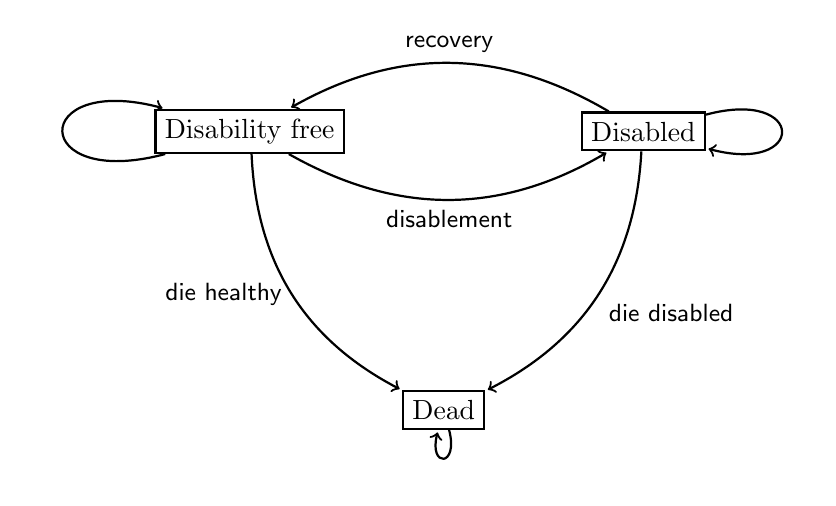
\begin{tikzpicture}[->,shorten >=1pt,auto,node distance=5cm,
  thick,main node/.style={draw}]

  \node[main node] (1) {Disability free};
  \node[main node] (2) [right of=1] {Disabled};
  \node[main node] (3) [below left of=2,xshift=1cm] {Dead};

  \path[every node/.style={font=\sffamily\small}]
    (1) edge [bend right] node [left] {die healthy} (3)
    (1) edge [bend right] node [below] {disablement} (2)
    (1) edge [loop left] node {} (1)
    (2) edge [bend right] node [above] {recovery} (1)
    (2) edge [loop right] node {} (2)
    (2) edge [bend left] node {die disabled} (3)
    (3) edge [loop below] node {} (3);
    
\end{tikzpicture}\\

\caption{State space for healthy and at least one ADL disability.}\label{fig:statespace}
\end{figure}

\section{Trends}

\begin{figure}
\centering
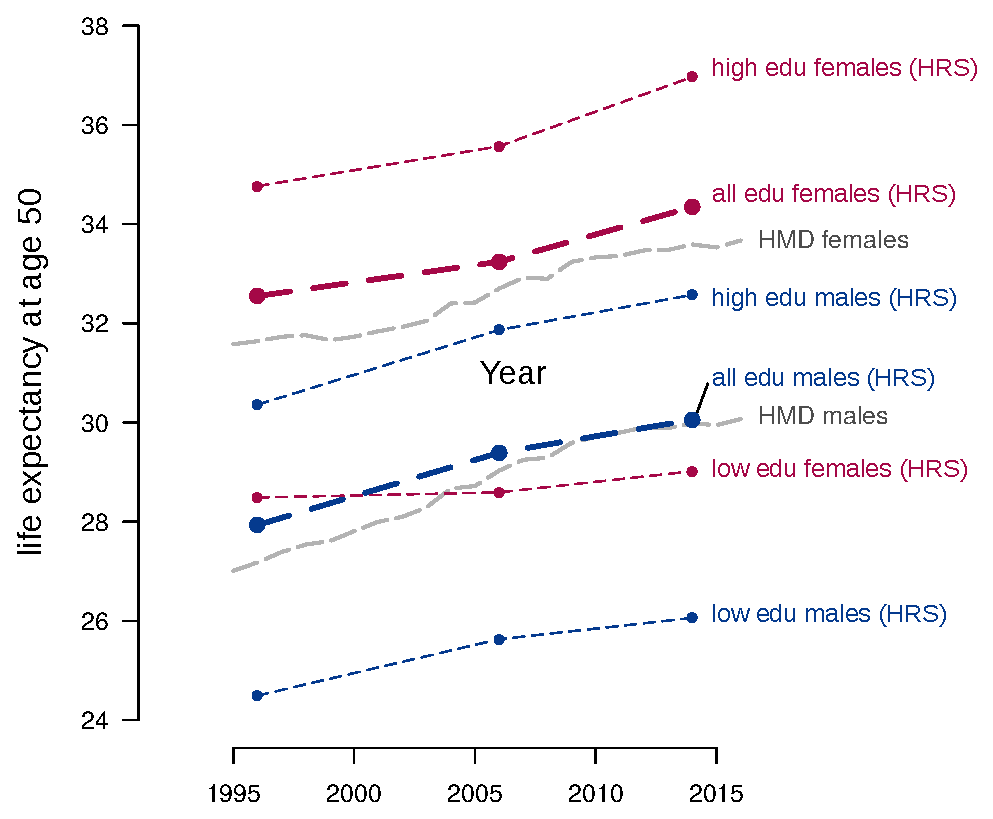
\includegraphics[scale=.7]{Figures/e50_Ink.pdf}
\end{figure}

\section{Model overview}
 In the specification presented at REVES (and discussed here) we have age as a spline with 3 knots, and it seems to behave reasonably well.\footnote{Due to discussion with Hiram Beltran Sanchez and NM, we may decide to move back to 4 knots to get more flexbility in younger ages.} There are controls for 4 race/eth categories, and strata for sex and 3 education groups\footnote{3 edu groups inherited from Jo's good judgement}. The group ``all edu'' refers to a statistical average edu, and all results refer to an artificial statistical average race/eth. We use the same proportion healthy and disabled at age 50 for all estimated variants. This would affect between-group comparisons (which we don't yet do), and it likely also affects the time trend, but we sweep it under the rug for now. Holding the proportions constant at age 50 in a sense makes all differences due to transition rates above 50, but that may be an incomplete accounting. We could hypthetically have group and time varying state proportions at age 50, and include these in the decompositions. Now for some discussion of the decomposition results.

\section{Rehash results}
This is a tabular representation of the decompositon results that were represented as bar charts in the REVES talk. I think it took too much mental gymnastics at REVES to realize the various ways in which things are additive, but it is actually quite clear in the following tables, since we have marginal sums, and people are used to such tables. First, we have a pretty good match to the HMD LE trend for the US (not shown).\footnote{Potential departures could be due to several understandable factors, and can be explained if necessary, but it's not worth gettign sidetracked by that just now.}. 

The main goods are the decompositions of the within-group changes between our present 3 time points (1996, 2006, 2014). Those time points are willy nilly, and we may move to annual estimates soon, so we can select years at-will. First, note that the columns DFLE and DLE sum to LE, both within changes due to transiton rates and within state expectancy changes. To interpret signs, it helps to moralize some: We \emph{want}: mortality down (DFLE +, DLE +), transitions to disability down (DFLE+, DLE-), and recovery up (DFLE+, DLE-).

The total change in male LE from \textbf{1996 to 2006} was 1.41, of which 1.27 came from an overall increase of 1.27 in DFLE. Looking at the LE column, we see that transitions from healthy to dead (m14) account for most of the change. Looking at the DLE column, we see that most increases were also due to the decreased mortality of healthy people (m14), but this was offset almost entirely by decreaed entries to disability (m12), not bad! The mortality of the disabled also improved a bit, adding .09 to DLE, .07 to DFLE (by allowing people to cycle back by not dying), adding to .15 LE, also a good outcome.

The total change in male LE from \textbf{2006 to 2014} was .65, of which .38 came from an increase in DFLE, and .27 from DLE, a less optimal breakdown. Looking at the LE column, we see that transitions from healthy to dead (m14) account for most of the change. The other story in this table is reduced recovery, which of course steals more healthy years than it adds disabled years. The other two factors increasing DLE are things that are actually quite good: they survive better, as do healthy people, allowing them to become disabled. Transitions into disability actually decreased. So, although DLE increased, most of the story behind it is straight good news: we just know that recovery is the only setback. Make sense?
\begin{table}[!ht]
      \caption{Males (all edu)}
      \label{tab:males}
      \centering
\subfloat[][1996-2006]{
      \begin{tabular}{rrr|r}
      \input{Data/Tables/mspec06/m-1996-2006-all.tex}
     \end{tabular}
}
     \qquad
\subfloat[][2006-2014]{
      \begin{tabular}{rrr|r}
      \input{Data/Tables/mspec06/m-2006-2014-all.tex}
     \end{tabular}
}
\end{table}

For females from \textbf{1996 to 2006} there was a modest gain in LE of .76 years, due to a strong increase in DFLE, partially offset by a decrease in DLE. Sounds like a good tradeoff until we realize that the reduction in DLE was due to i) worse mortality and ii) worse recovery. At the same time transitions to disability decreased, adding .73 to DFLE and deducting .43 from DLE- that's straight good news, but transitinos out of disability were straight bad news. This is not the way to engineer compression folks. The main protagonist here is again improved mortality of the healthy.

For females from \textbf{2006 to 2014} we have a strong increase in LE of 1.47 years, due entirely to mortality (1.36+.54), mostly the mortality of the healthy. Recovery got way worse (-.93,+.51)and onset was unchanged. This lead to a large increase in DLE and a merely modest increase in DFLE: so large was the recovery setback (-.93) that it almost entirely chancelled out the good news for the mortality of the healthy (+.98). If we could ignore ``health dynamics'', we would have had something like dynamic equilibrium in this period, but althogether this is straight expansion, boo.

\begin{table}[!ht]
      \caption{Females (all edu)}
      \label{tab:females}
      \centering
\subfloat[][1996-2006]{
      \begin{tabular}{rrr|r}
      \input{Data/Tables/mspec06/f-1996-2006-all.tex}
     \end{tabular}
}
     \qquad
\subfloat[][2006-2014]{
      \begin{tabular}{rrr|r}
      \input{Data/Tables/mspec06/f-2006-2014-all.tex}
     \end{tabular}
}
\end{table}

There are obvious ways to frame these results in a compression, expansion, equilibrium language. That may be nice because it's familiar language. To be clear it would be possible to decompose with respect to a clear measure of compression (DLE / LE), but I do prefer to keep things in year units.

It would also be possible to plug in some counterfactuals to guage better what levers are the closest at hand. In the way things are now, it would seem to pay off nicely to invest in recovery: improvements in recovery adds more to DFLE than it subtracts from DLE. This is probably truer the greater the mortality gradient between states. I've also asked DCS to add a state ``healthy but ever disabled'', as a check on the homogeneity of the healthy-- this is necessary to know how realistic the recovery payoff, as stated above, is. It would change the arrow configuration in the state space too (no returns to straight good health).
% bibliography
%\bibliographystyle{spbasic}
%\bibliography{references}  
\end{document}
